
%%%%%%%%%%%%%%%%%%%%%%% file typeinst.tex %%%%%%%%%%%%%%%%%%%%%%%%%
%
% This is the LaTeX source for the instructions to authors using
% the LaTeX document class 'llncs.cls' for contributions to
% the Lecture Notes in Computer Sciences series.
% http://www.springer.com/lncs       Springer Heidelberg 2006/05/04
%
% It may be used as a template for your own input - copy it
% to a new file with a new name and use it as the basis
% for your article.
%
% NB: the document class 'llncs' has its own and detailed documentation, see
% ftp://ftp.springer.de/data/pubftp/pub/tex/latex/llncs/latex2e/llncsdoc.pdf
%
%%%%%%%%%%%%%%%%%%%%%%%%%%%%%%%%%%%%%%%%%%%%%%%%%%%%%%%%%%%%%%%%%%%

\documentclass[runningheads,a4paper]{llncs}
\usepackage{amssymb}
\setcounter{tocdepth}{3}
\usepackage{graphicx}
\usepackage[subrefformat=parens,labelformat=parens]{subfig}
\usepackage{algorithm}
\usepackage{algpseudocode}
\usepackage{footnote}
\usepackage{multirow}
%\usepackage{mathptmx}
%\usepackage{amsmath}
\usepackage{url}


\urldef{\mailsa}\path|{alfred.hofmann, ursula.barth, ingrid.haas, frank.holzwarth,|
	\urldef{\mailsb}\path|anna.kramer, leonie.kunz, christine.reiss, nicole.sator,|
	\urldef{\mailsc}\path|erika.siebert-cole, peter.strasser, lncs}@springer.com|    
\newcommand{\keywords}[1]{\par\addvspace\baselineskip
	\noindent\keywordname\enspace\ignorespaces#1}

\def\D{\mathrm{d}}


\newenvironment{mycell}[1]
{
	\begin{minipage}{#1}
		\begin{center}
			\vspace*{0.15cm}
		}
		{
			\vspace*{0.1cm}
		\end{center}
	\end{minipage}
}
\newenvironment{mycellS}[1]
{
	\begin{minipage}{#1}
		\begin{center}
		}
		{
			\vspace*{0.01cm}
		\end{center}
	\end{minipage}
}
\newenvironment{leftcell}[1]
{
	\begin{minipage}{#1}
		\begin{flushleft}
			\vspace*{0.15cm}
		}
		{
			\vspace*{0.1cm}
		\end{flushleft}
	\end{minipage}
}

\newenvironment{equationexp}[1]% Environment for explaining equation variables
{\begin{list}{}%
		{\setlength{\leftmargin}{#1}}%
		\item[]%
	}
	{\end{list}}
\DeclareGraphicsExtensions{.tif,.jpg,.pdf,.mps,.png}
\graphicspath{{./pic/}} % PUT ALL PDF/JPG/PNG FIGURES IN THIS SUBDIR
\graphicspath{{./jpeg/}} % PUT ALL PDF/JPG/PNG FIGURES IN THIS SUBDIR
\begin{document}
	
	\mainmatter  % start of an individual contribution
	
	% first the title is needed
	\title{Noisy Softplus: A Biology Inspired Activation Function}
	
	% a short form should be given in case it is too long for the running head
	\titlerunning{Noisy Softplus: A Biology Inspired Activation Function}
	
	% the name(s) of the author(s) follow(s) next
	%
	% NB: Chinese authors should write their first names(s) in front of
	% their surnames. This ensures that the names appear correctly in
	% the running heads and the author index.
	%
	\author{Qian Liu \and Steve Furber
		%	\thanks{Please note that the LNCS Editorial assumes that all authors have used the western naming convention, with given names preceding surnames. This determines	the structure of the names in the running heads and the author index.}%
	}
	%
	\authorrunning{Qian Liu \and Steve Furber}
	% (feature abused for this document to repeat the title also on left hand pages)
	
	% the affiliations are given next; don't give your e-mail address
	% unless you accept that it will be published
	\institute{Advanced Processor Technologies group, School of Computer Science,\\
		University of Manchester, M13 9PL, Manchester, United Kingdom\\
		{qian.liu-3, steve.furber}@manchester.ac.uk
		%\mailsa\\
		%\mailsb\\
		%\mailsc\\
		%\url{http://www.springer.com/lncs}
	}
	
	%
	% NB: a more complex sample for affiliations and the mapping to the
	% corresponding authors can be found in the file "llncs.dem"
	% (search for the string "\mainmatter" where a contribution starts).
	% "llncs.dem" accompanies the document class "llncs.cls".
	%
	
	\toctitle{Lecture Notes in Computer Science}
	\tocauthor{Authors' Instructions}
	\maketitle
	
	
	\begin{abstract}
		The Spiking Neural Network (SNN) has not achieved the recognition/classification performance of its non-spiking competitor, the Artificial Neural Network(ANN), particularly when used in deep neural networks.
		The mapping of a well-trained ANN to an SNN is a hot topic in this field, especially using spiking neurons with biological characteristics.
		This paper proposes a new biologically-inspired activation function, Noisy Softplus, which is well-matched to the response function of LIF (Leaky Integrate-and-Fire) neurons.
		A convolutional network (ConvNet) was trained on the MNIST database with Noisy Softplus units and converted to an SNN while maintaining a close classification accuracy.
		This result demonstrates the equivalent recognition capability of the more biologically-realistic SNNs and bring biological features to the activation units in ANNs.
		\keywords{Noisy Softplus, biologically-inspired, Spiking Neural Network, activation function, LIF neurons}
	\end{abstract}
	
	\section{Introduction}
	%Spiking Neural Network (SNN) has not achieved the recognition/classification performance of its non-spiking competitor, ANN.
	
	Deep Neural Networks (DNNs) are the most promising research field in computer vision, even exceeding human-level performance on image classification tasks~\cite{he2015delving}.
	To investigate whether brains might work similarly on vision tasks, these powerful DNN models have been converted to spiking neural networks (SNNs).
	In addition, the spiking DNN offers the prospect of neuromorphic systems that combine remarkable performance with energy-efficient training and operation.
	
	Theoretical studies have shown that biologically-plausible learning, e.g. Spike-Timing-Dependent Plasticity (STDP), could approximate a stochastic version of powerful machine learning algorithms
%	~\cite{nessler2013bayesian,neftci2013event,neftci2013event,o2016deep}.
	such as 
%	Expectation Maximization~\cite{nessler2013bayesian}, 
	Contrastive Divergence~\cite{neftci2013event}, Markov Chain Monte Carlo~\cite{buesing2011neural} and Gradient Descent~\cite{o2016deep}.
	Stochasticity, in contrast with the continuously differentiable functions used by ANNs, is intrinsic to the event-based spiking process, making network training difficult.
	In practice, ANNs use neuron and synapse models very different from biological neurons, and it remains an unsolved problem to develop SNNs with equivalent performance.
	
	%How to map a well trained ANN to SNN is a hot topic in this field, especially using spiking neurons of biological scale.
	
	On the other hand, the offline training of an ANN, which is then mapped to an SNN, has shown near loss-less conversion and state-of-the-art classification accuracy.
	This research aims to prove that SNNs are equally capable as their non-spiking rivals of pattern recognition, and at the same time are more biologically realistic and energy-efficient.
	Jug et. al.~\cite{Jug_etal_2012} first proposed the use of the Siegert function to replace the sigmoid activation function in Restricted Boltzmann Machine (RBM) training.
	The Siegert units map incoming currents driven by Poisson spike trains to the response firing rate of a Leaky Integrate-and-Fire (LIF) neuron.
	The ratio of the spiking rate to its maximum is equivalent to the output of a sigmoid neuron.
	A spiking Deep Belief Network (DBN)~\cite{Stromatias2015scalable} was implemented on neuromorphic hardware, SpiNNaker~\cite{furber2014spinnaker}, to recognise hand written digits in real time.
	However, cortical neurons seldom saturate their firing rate.
	Thus Rectified Linear Units (ReLU) were proposed and surpassed the performance of other popular activation units thanks to their advantage of sparsity~\cite{glorot2011deep}.
	Recent work~\cite{hunsberger2015spiking} proposed the Soft LIF response function, which is equivalent to Softplus activation.
%	~\cite{dugas2001incorporating}.
	%trained with noisy input, the 4-layered spiking autoencoder reached 98.37\% accuracy on MNIST. 
	
	Even better performance~\cite{cao2015spiking,diehl2015fast} has been demonstrated in Spiking Convolutional Networks (ConvNets), but this employed simple integrate and fire neurons.
	The training used only ReLUs and zero bias to avoid negative outputs, and applied a deep learning technique, dropout, to increase the classification accuracy.
	Normalising the trained weights for use on an SNN was relatively straightforward and maintained the classification accuracy.
	This work was extended to a Recursive Neural Network (RNN)~\cite{diehl2016conversion} and run on the TrueNorth~\cite{merolla2014million} neuromorphic hardware platform.
	
	The Noisy Softplus activation function proposed here is based on LIF neurons with biological characteristics, and is the first attempt to map a spiking neural response accurately to the activation unit of an ANN.
	The resulting classification accuracy was tested on a spiking ConvNet; the performance was close to that of the original ConvNet, and was better than using Softplus.
	This study brings a significant biological feature, noise, to the activation units of an ANN, in the hope of promoting research into noise-based computation.
	
	\section{Methods}
	\subsection{Neural Science Background}
	%As discussed above, most of the top scored networks map the ReLUs in ANN to the equivalent spiking version of IF neurons.
	This paper proposes a new activation function, Noisy Softplus, which is inspired by neuroscience observations of LIF neurons.
	The LIF neuron model follows the following membrane potential dynamics:
	\begin{equation}
	\tau_m \frac{\D V}{\D t}=V - V_{rest} + R_{m} I(t) ~.
	\label{eq:LIF}
	\end{equation}
	The membrane potential $V$ changes in response to the input current $I$, starting at the resting membrane potential $V_{rest}$, where the membrane time constant is $\tau_m = R_mC_m$, $R_m$ is the membrane resistance and $C_m$ is the membrane capacitance.
	The central idea in converting spiking neurons to activation units lies in the response function of a neuron model.
	Given a constant current injection $I$, the response function, i.e. firing rate, of the LIF neuron is:
	\begin{equation}
	\lambda_\mathit{out}=
	\left [ t_\mathit{ref}-\tau_m\log \left ( 1-\frac{V_{th}-V_\mathit{rest}}{IR_m}  \right )\right ]^{-1}, \textrm{~when~} IR_m>V_{th}-V_{rest},
	\label{equ:consI}
	\end{equation}
	otherwise the membrane potential cannot reach the threshold $V_{th}$ and the output firing rate is zero. 
	The absolute refractory period $t_\mathit{ref}$ is included, where all input during this period is ignored.
	The dotted (zero noise) line in Fig.\subref*{Fig:physics} illustrates the response function of an LIF neuron, which inspired the proposal of ReLUs.
	The parameters of the LIF neuron are all biologically valid (see the listed values in Table~\ref{tbl:pynnSetting}), and the same parameters are used throughout this paper.
	In practice, a noisy current generated by the arrival of spike trains, rather than a constant current, flows into the neurons.
	The response function
%	~\cite{la2008response}
	of the LIF neuron to a noisy current is as follows, where $\mu$ and $\sigma$ are the mean and variance of the current:
	\begin{equation}
	\lambda_\mathit{out}=
	\left [ t_\mathit{ref}+\tau_m \int_{\frac{V_\mathit{rest}-\mu \tau_m }{\sigma \sqrt{\tau_m}}}^{\frac{V_{th}-\mu \tau_m }{\sigma \sqrt{\tau_m}}} \sqrt{\pi} \exp(u^{2}) (1+erf(u)) \D u \right ]^{-1} ~.
	\label{equ:noiseI}
	\end{equation}
	
	\begin{figure}[bt!]
		\centering
		\subfloat[Response function with noisy currents.]{
			\label{Fig:physics}
			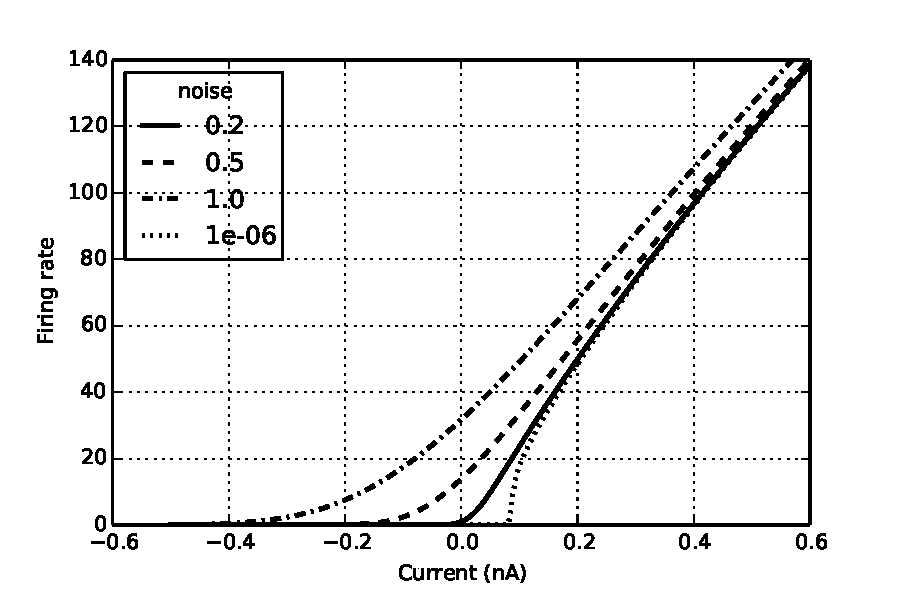
\includegraphics[width=0.5\textwidth]{pic/1.pdf}
		}
		\subfloat[Recorded response firing rate.
		%	 of the LIF neuron.
		%		The simulation is done using NoisyCurrentSource supported by PyNN and run on Nest~\cite{gewaltig2007nest}.
		%		The neuron is driven by a noisy current with different standard deviations. 
		]{
			\label{Fig:lif_curr}
			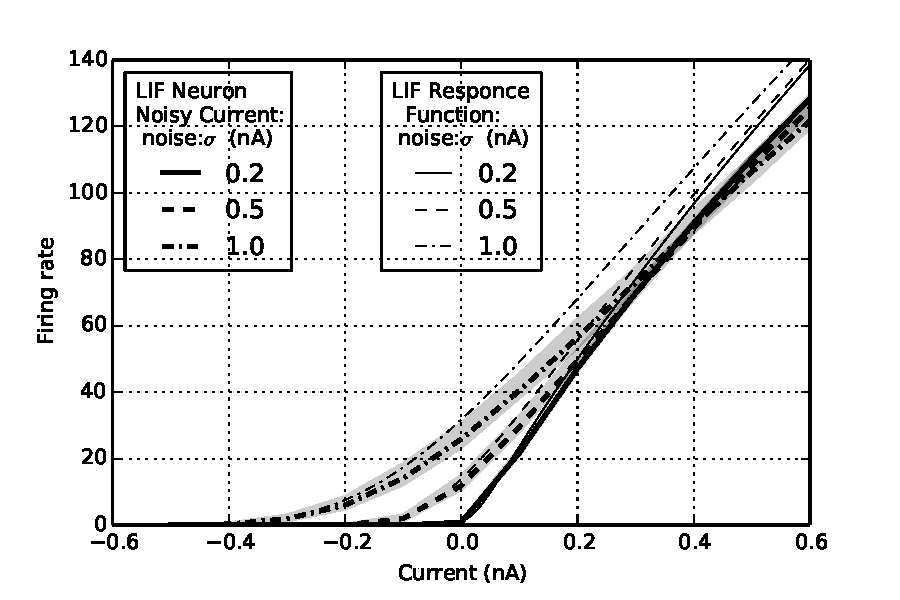
\includegraphics[width=0.5\textwidth]{pic/2.pdf}
		}
		\caption{
			(a) Response function of the LIF neuron with noisy input currents with different standard deviations.
			(b) Comparing the recorded firing rates of the LIF neuron simulation driven by noisy currents to the response function shown in (a). }
		\label{fig:firefunc}	
	\end{figure}
	\begin{table}[bt]
		\centering
		\caption{\label{tbl:pynnSetting}Parameter setting for the current-based LIF neurons using PyNN.}
		\bgroup
		\def\arraystretch{1.4}
		\begin{tabular}{c|| c |c| c| c| c| c| c| c}
			%		%\hline
			%		Parameters & Values & Units \\
			%		\hline
			%		cm & 0.25 & nF	\\
			%		%\hline
			%		tau\_m & 20.0 & ms\\
			%		%\hline
			%		tau\_refrac & 1.0 & ms\\
			%		%\hline
			%		tau\_syn\_E & 5.0 & ms\\
			%		%  %\hline
			%		tau\_syn\_I & 5.0 & ms\\
			%		%  %\hline
			%		v\_reset & -65.0 & mV\\
			%		%\hline
			%		v\_rest & -65.0 & mV\\
			%		%\hline
			%		v\_thresh & -50.0 & mV\\
			%		%\hline
			%		i\_offset & 0.1 & nA\\
			\hline
			Parameters & cm & tau\_m & tau\_refrac & tau\_syn\_E & tau\_syn\_I & v\_rest & v\_thresh & i\_offset \\
			Values & 0.25 &  20.0 & 1.0 & 5.0 & 5.0 & -65.0 & -50.0  & 0.1 \\
			Units & nF & ms & ms & ms & ms & mV & mV& nA\\
			\hline
		\end{tabular}
		\egroup
	\end{table}
	
	
	
	\subsection{LIF Neuron Simulation}
	To verify the response function, a simulation was carried out using PyNN~\cite{davison2008pynn} to compare with the analytical results.
	A noisy current with a particular $\mu$ and $\sigma$ was injected into an LIF neuron for 10~s.
	The firing rate was the average among 10 trials, see Fig.\subref*{Fig:lif_curr}.
	The slight difference compared to the analytical results (dashed lines) comes from the time resolution of the simulated noisy current.
	A more realistic simulation of a noisy current is generated by a Poisson spike train, 
	%assuming that large amount of small amplitude PSPs are required to reach the threshold and $\tau_syn$ limits to 0.
	where the mean and variance are given by:
	\begin{equation}
	\mu = \tau_{syn}\sum_i w_i\lambda_{i}~,~\sigma^2=\frac{1}{2}\tau_{syn}\sum_i w_i^2\lambda_{i}~,
	\end{equation}
	where $\tau_{syn}$ is the synaptic time constant, and each Poisson spike train connects to the neuron with a strength of $w_i$ and a firing rate of $\lambda_i$.
	Two populations of Poisson spike sources, for excitatory and inhibitory synapses respectively, were connected to a single LIF neuron to mimic the noisy currents.
	The firing rates of the Poisson spike generators were determined by the given $\mu$ and $\sigma$.
	Fig.~\ref{fig:lif_pois} illustrates the recorded firing rates responding to the spike trains compared to the result driven by noisy currents.
	The use of noisy currents assumes that the post-synaptic potential (PSP) is a delta function, e.g. $\tau_{syn}$ tends to the limits of 0.
	However, in practice the release of neurotransmitter takes time and the noise added to the mean current is not pure white noise.
	Thus the experiments show that a longer $\tau_{syn}$ increases the level of noise and widens the variance of the output firing rate.
	
	\begin{figure}[bt!]
		\centering
		\subfloat[$\tau_{syn}=1$~ms]{
			\label{Fig:lif_pois1}
			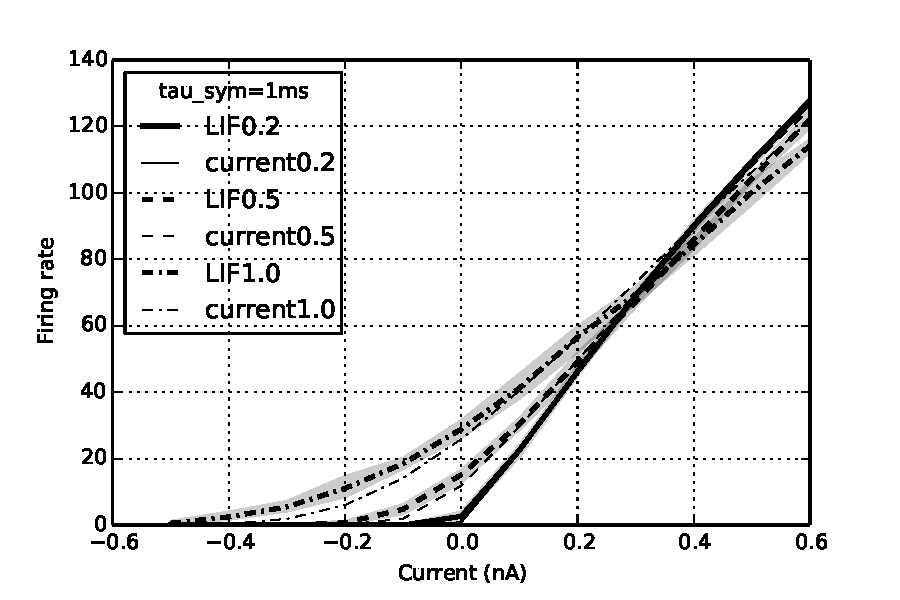
\includegraphics[width=0.5\textwidth]{pic/3-1.pdf}
		}
		\subfloat[$\tau_{syn}=5$~ms]{
			\label{Fig:lif_pois5}
			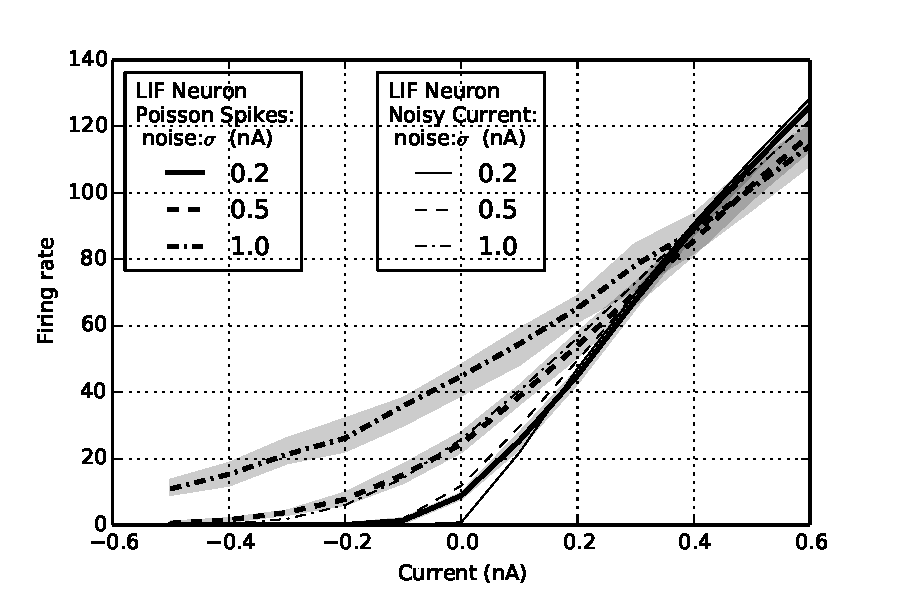
\includegraphics[width=0.5\textwidth]{pic/3-2.pdf}
		}
		\caption{
			Recorded response firing rate of two LIF neurons with different synaptic constants.
			The driving noisy current is simulated with Poission spike trains and the results are compared to the noisy current source.}
		\label{fig:lif_pois}	
	\end{figure}
	
	\begin{figure}[htb!]
		\centering
		%	\subfloat[Noisy Softplus.]{
		%		\label{Fig:sp}
		%		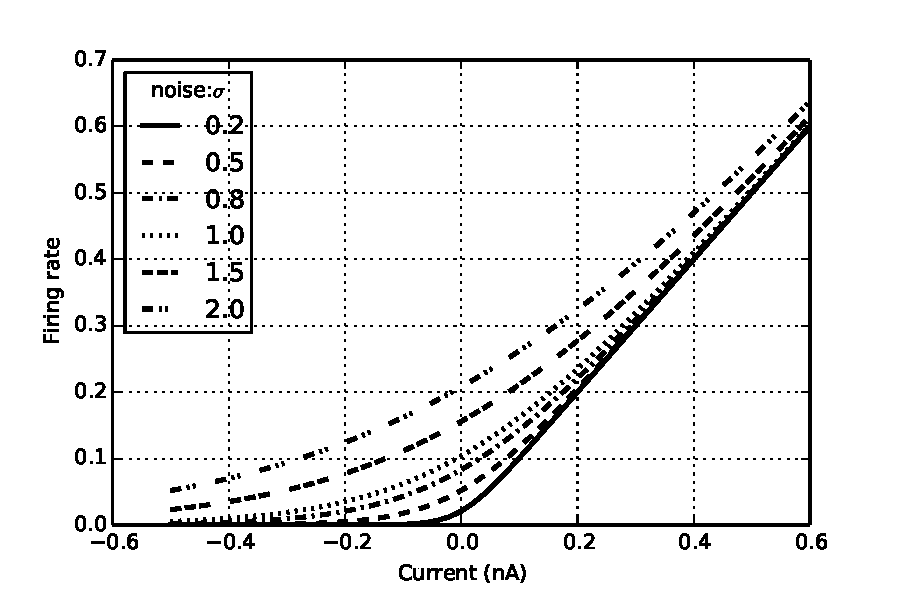
\includegraphics[width=0.5\textwidth]{pic/4.pdf}
		%	}
		\subfloat[Noisy Softplus]{
			\label{Fig:nsp}
			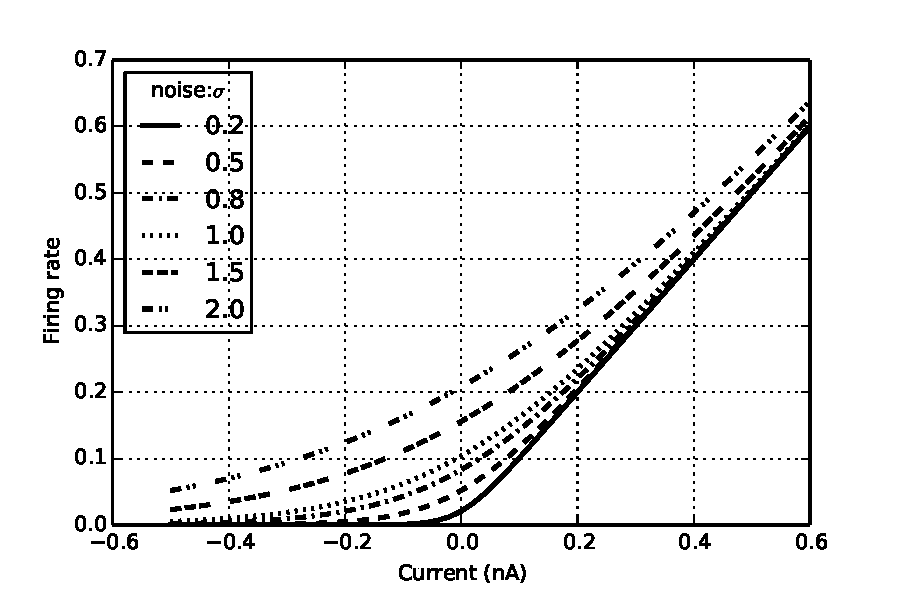
\includegraphics[width=0.5\textwidth]{pic/4.pdf}
		}
		\subfloat[Noisy Softplus in 3D]{
			\label{Fig:3d}
			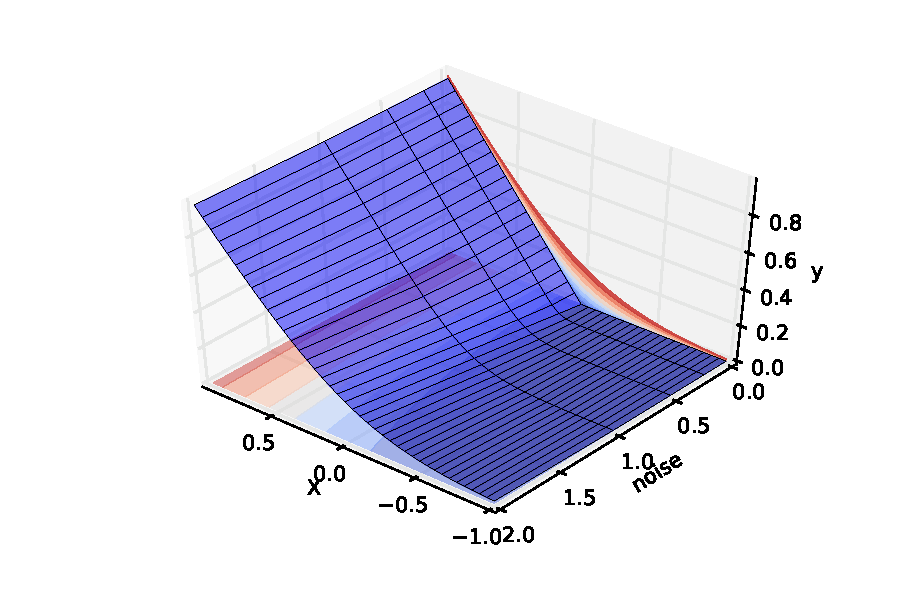
\includegraphics[width=0.45\textwidth]{pic/5.pdf}
		}\\
		\subfloat[$k=0.17$ and $\tau_{syn}=1$~ms]{
			\label{Fig:nsptau1}
			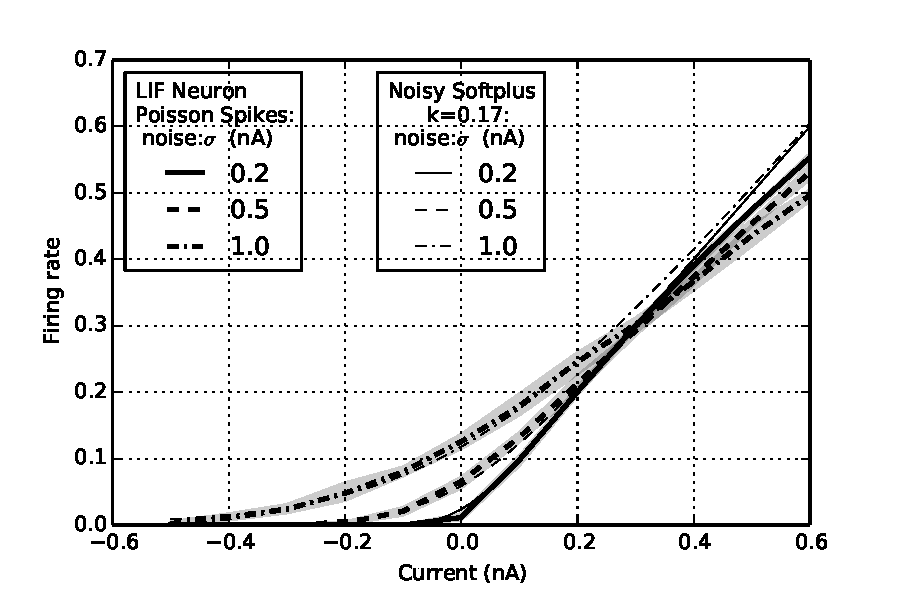
\includegraphics[width=0.5\textwidth]{pic/4-1.pdf}
		}
		\subfloat[$k=0.3$ and $\tau_{syn}=5$~ms]{
			\label{Fig:scale}
			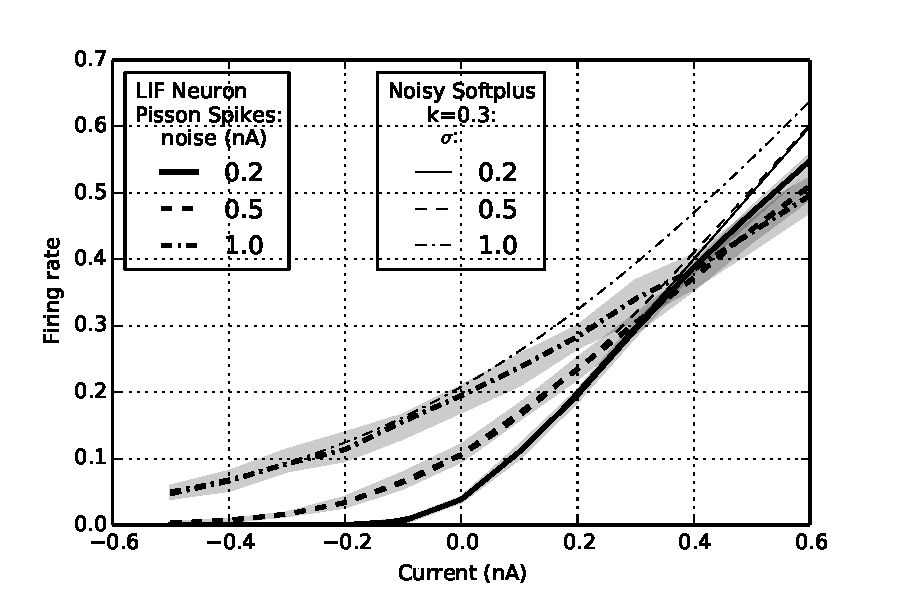
\includegraphics[width=0.5\textwidth]{pic/4-2.pdf}
		}
		\caption{
			Noisy Softplus fits to the response function of the LIF neuron.
			Noisy Softplus in (a) curve sets and (b) 3D.
			(c) and (d) show how Noisy Softplus fits to the response firing rates of LIF neurons with different synaptic constants.}
		\label{fig:nsp}
	\end{figure}
	
	\subsection{Noisy Softplus}
	Inspired by the set of response functions triggered by different levels of noise, we propose the Noisy Softplus activation function:
	\begin{equation}
	y = f_{ns}(x, \sigma) = k \sigma \log [1 + \exp(\frac{x}{k \sigma})],
	\label{equ:nsp}
	\end{equation}
	where $x$ refers to the mean current, $y$ is the normalised output firing rate, $\sigma$ plays an important role to define the noise level, and $k$, which is determined by the neuron parameters, controls the curve scaling.
	Note that the novel activation function we propose contains two parameters, the current and its noise; both are naturally obtained in spiking neurons.
	% With doubled information, more powerful training methods and network models are expected. 
	Fig.\subref*{Fig:nsp} and \subref*{Fig:3d} show the activation function in curve sets and in a 3D plot.
	The Noisy Softplus fits well to the recorded response firing rate of the LIF neuron with suitable calibration of $k$, see Fig.\subref*{Fig:nsptau1} and \subref*{Fig:scale}.
	The derivative is the logistic function scaled by $k\sigma$:
	\begin{equation}
	\frac{\partial f_{ns}(x,\sigma)}{\partial x} = \frac{1}{1+exp(-\frac{x}{k\sigma})}.
	\label{equ:logist}
	\end{equation}	
	
	\begin{figure}[bt!]
		\centering
		\subfloat[Pixel firing rates]{
			\label{Fig:62}
			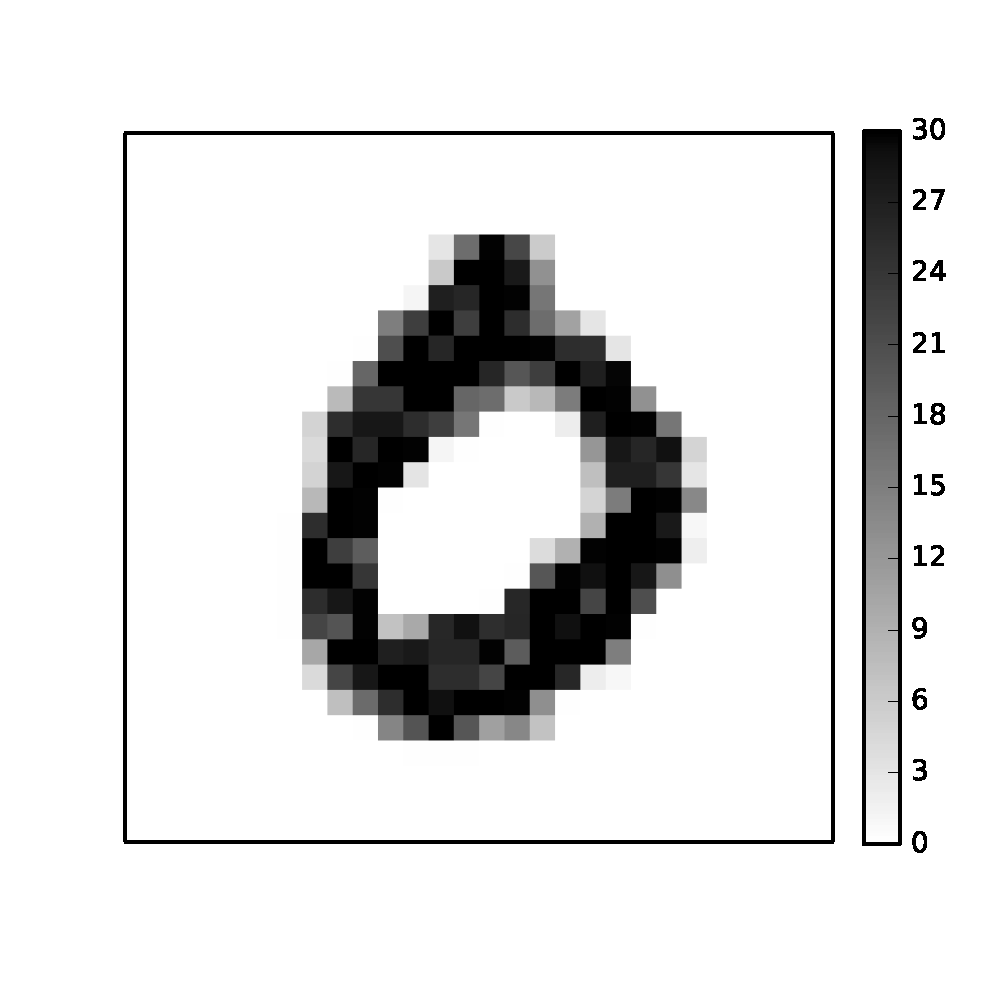
\includegraphics[width=0.3\textwidth]{pic/6-2.png}
		}
		\subfloat[5x5 kernel]{
			\label{Fig:63}
			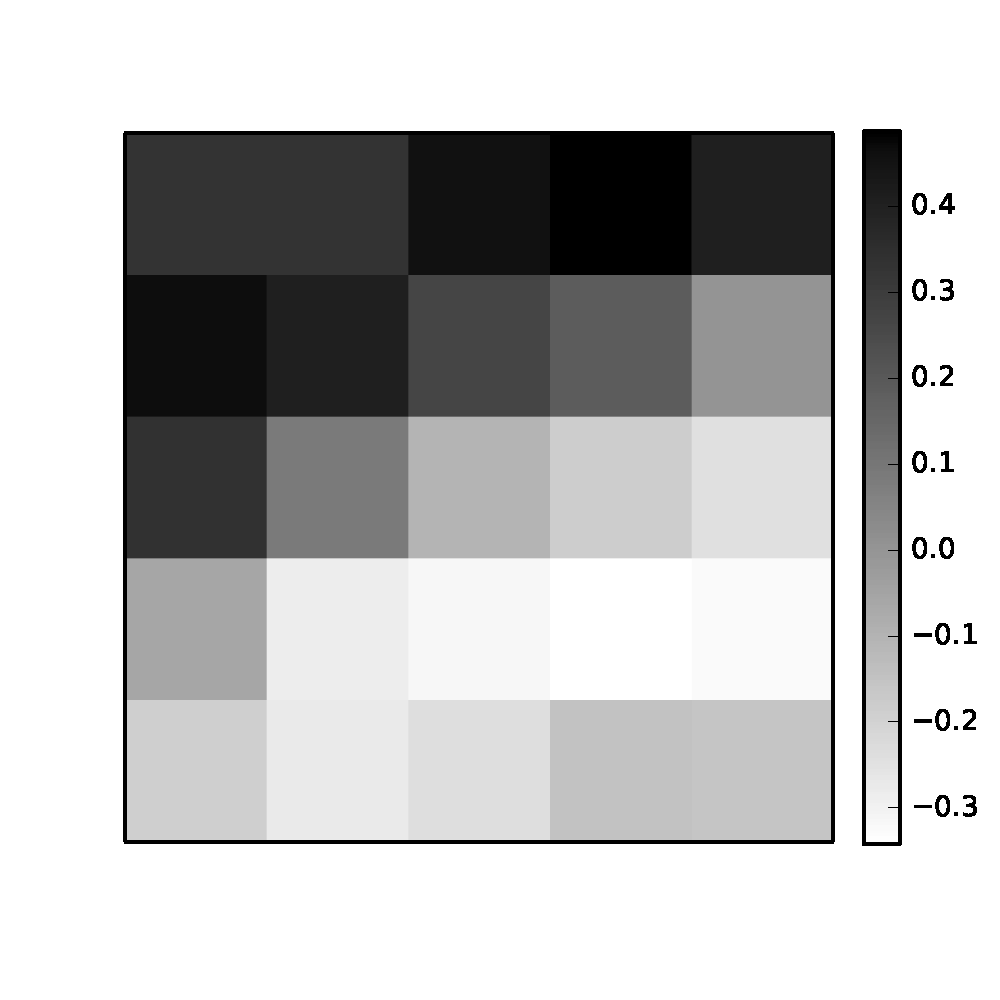
\includegraphics[width=0.3\textwidth]{pic/6-3.png}
		}
		\subfloat[Output firing rates]{
			\label{Fig:64}
			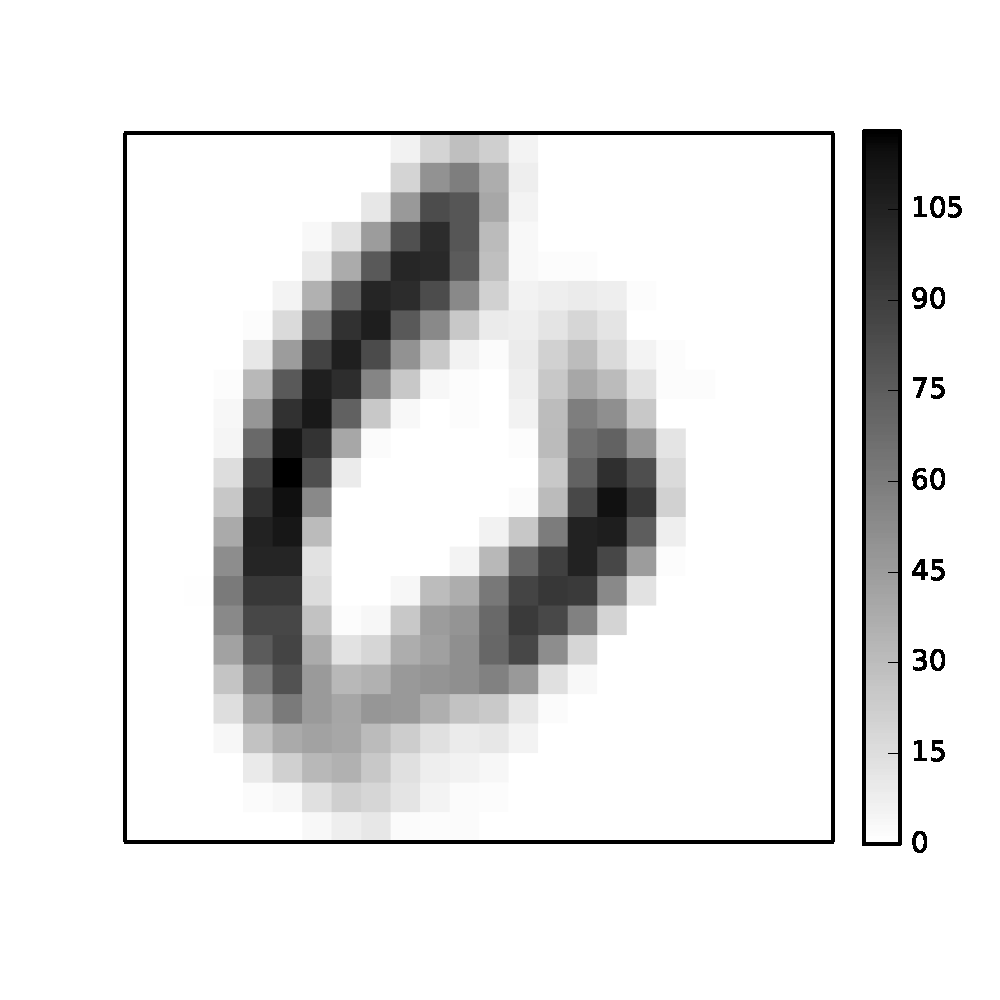
\includegraphics[width=0.3\textwidth]{pic/6-4.png}
		}
		\\
		\subfloat[10 input digits as a raster plot]{
			\label{Fig:61}
			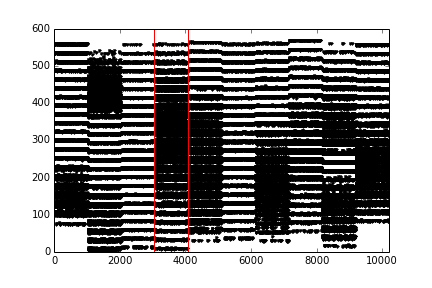
\includegraphics[width=0.5\textwidth]{pic/6-1.png}
		}
		\subfloat[Observed `activation functions']{
			\label{Fig:65}
			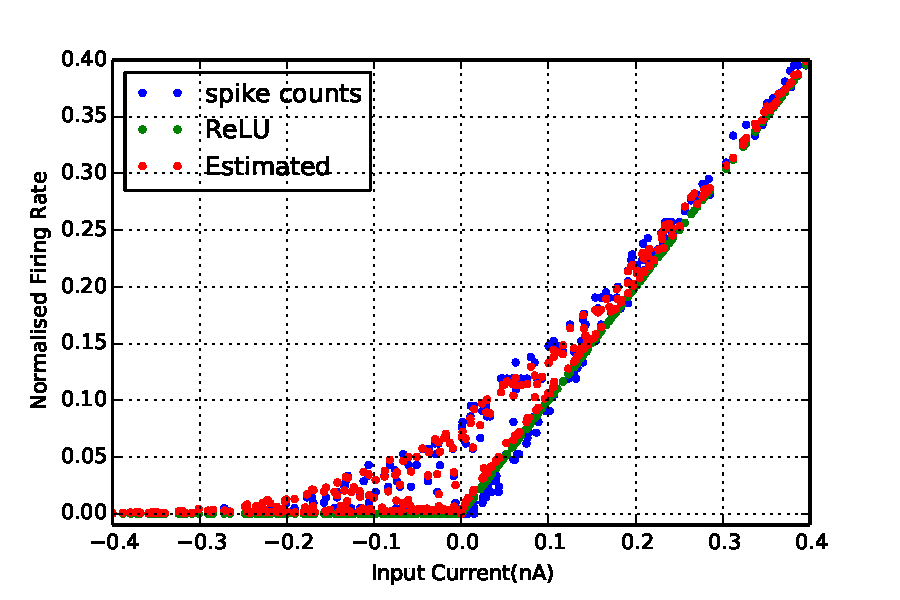
\includegraphics[width=0.5\textwidth]{pic/6-5.pdf}
		}
		\caption{
			Noisy Softplus fits to the neural response firing rate in an SNN simulation.
			The 28x28 Poisson spike trains in (a) firing rate, and (d) raster plots, are convolved with a 5x5 kernel (b).
			(c) the convolved map with the firing rates of each neuron.
			(e) the normalised firing rate compared with Noisy Softplus, Softplus and ReLU activation functions.}
		\label{fig:cnn}
	\end{figure}
	
	\section{Results}
	A ConvNet model was trained on MNIST,
%	~\cite{lecun1998gradient}
	a popular database in neuromorphic vision, using Noisy Softplus neurons.
	The architecture contains 28x28 input units, followed by two convolutional layers c5-2s-12c5-2s, and the 10 output neurons represents the classified digit.
	All the convolution and average sampling neurons use Noisy Softplus units with no bias, while the output neurons are softmax units converting a vector of values into the range (0, 1) that add up to 1.
	The weights were updated using a fixed learning rate, 50 images per batch and 10 epochs.
	Before testing on spiking LIF neurons, the weights of each layer were scaled to ensure that input synaptic currents stay within a valid range.
	
	To validate how well the Noisy Softplus activation fits to the response firing rate of LIF neurons in a real application, we simulated the model on Nest using the Poisson MNIST dataset~\cite{liu2016bench} and the neurons of a convolutional map were observed.
	Fig.~\ref{fig:cnn} shows the convolution of a 5x5 kernel with an input digit `0' represented by spike trains.
	The estimated spike counts using Noisy Softplus fit to the real recorded firing rate much more accurately than the Softplus and ReLU activation functions.
	In Fig.~\subref*{Fig:65}, we manually selected a suitable scaling factor for Softplus which located on the top slope of the response activity.
	However, the scale factor remains static for all the neurons, thus resulting in a mismatch at different level of noise.
	Noisy Softplus adapts to noise automatically.
	

	
	
	We compared the training using ReLU, Softplus, and Noisy Softplus by their loss during training averaged over 6 trials, see Fig.\ref{fig:training}.
	The trained networks were scaled to SNNs and compared on recognition rates, 93.34\%, 96.43\% and 97.03\% with a conversion loss of 4.76\%, 0.91\% and 0.74\%.
	As it is a major concern in neuromorphic vision, the recognition performance over short response times is also estimated in Fig.\subref*{Fig:response}.
	\begin{figure}[bt!]
		\centering
		\subfloat[Ouput firing rates]{
			\label{Fig:out}
			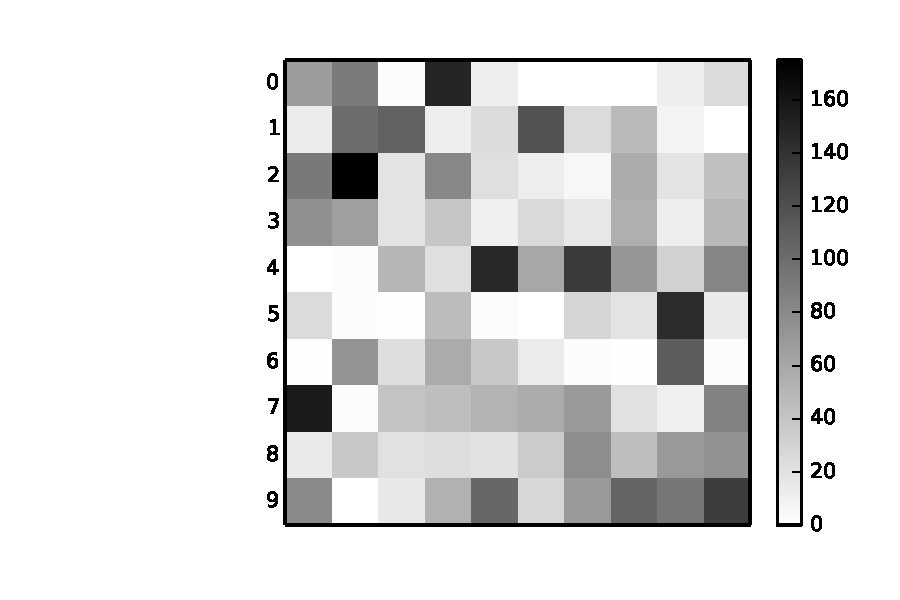
\includegraphics[width=0.26\textwidth]{pic/7.pdf}
		}
		\subfloat[Loss over training]{
			\label{Fig:loss}
			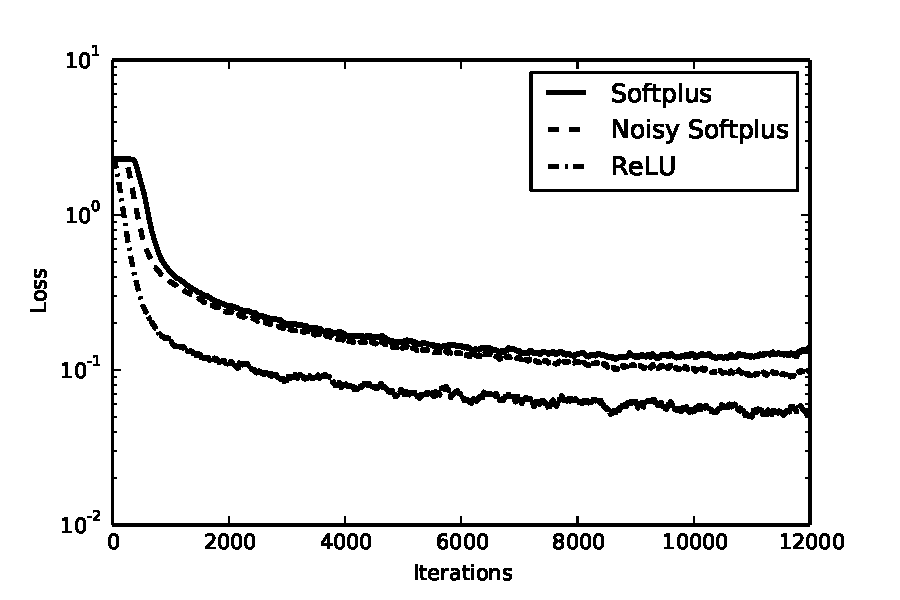
\includegraphics[width=0.35\textwidth]{pic/8.pdf}
		}
		\subfloat[Performance over time]{
			\label{Fig:response}
			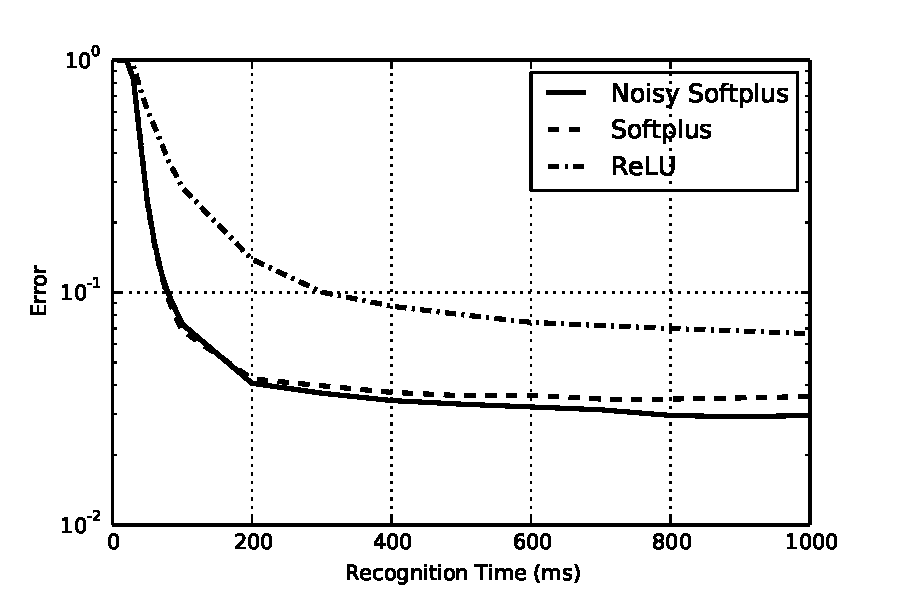
\includegraphics[width=0.35\textwidth]{pic/9.pdf}
		}
		\caption{
			Classification performance is calculated by the firing rate of output neurons (a).
			(b) shows how the loss varies over training.
			(c) illustrates the accuracy over short response times.}
		\label{fig:training}	
	\end{figure}
	
	%\begin{figure}[bt!]
	%	\centering
	%	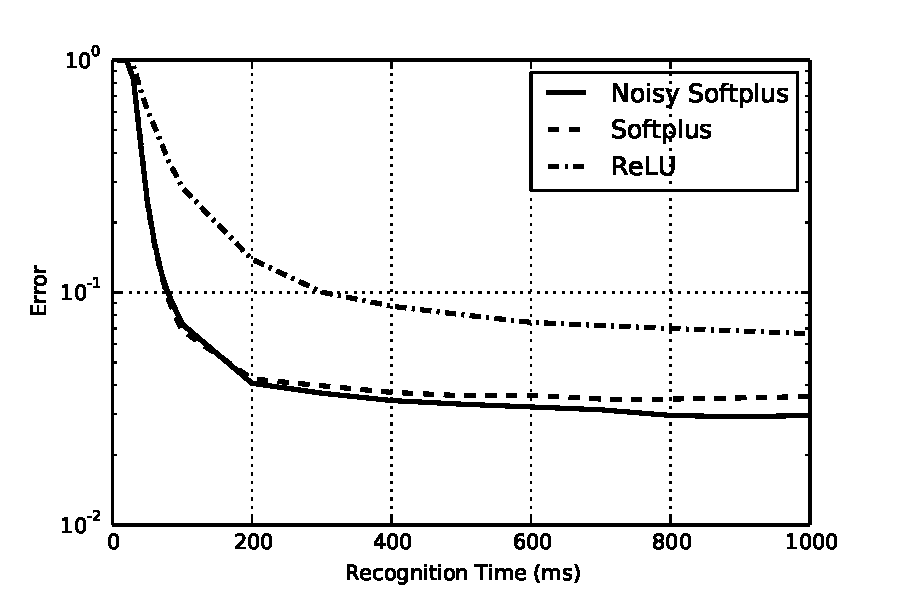
\includegraphics[width=0.75\textwidth]{pic/9.pdf}
	%	\caption{
	%	Classification accuracy varies over time.}
	%	\label{fig:response}	
	%\end{figure}
	
	\section{Discussion}
	The biologically-inspired activation function, Noisy Softplus, adapts to the noise level of input currents automatically, and is the first attempt to map activation units accurately to the firing response of LIF neurons.
	Noisy Softplus not only brings more biological features to the activation function, but also proves capable of performing well in a spiking ConvNet recognition task.
	The spiking version of Noisy Softplus wins on accuracy over the sigmoid neuron, compared to the result~\cite{Stromatias2015scalable} of using Siegert units.
	As a result of its more accurate mapping, Noisy Softplus outperforms Softplus.
	
	Future work on SNNs will include constraints during training to limit the function within the active range, which is equivalent to constraining the maximum firing rate of an LIF neuron.
	As a result there should be no need for the scaling process after training.
	For more accurate mapping, the scale factor $k$ should be (numerically) derived to avoid calibration.
	In ANNs, it could be useful to study noise as extra information to be gathered by Softplus activation to enhance classification.
	
	
	\section*{Acknowledgments}
	
	%The work presented in this paper was largely inspired by discussions at the 2015 Workshops on Neuromorphic Cognition Engineering in CapoCaccia.
	%The authors would like to thank the organisers and the sponsors.
	%The authors would also like to thank Patrick Camilleri, Michael Hopkins, and Viv Woods for meaningful discussions and proof-reading the paper.
	%The construction of the SpiNNaker machine was supported by the Engineering and Physical Sciences Research Council (EPSRC grant EP/4015740/1) with additional support from industry partners ARM Ltd and Silistix Ltd.
	The research leading to these results has received funding from the European Research Council 
%	under the European Union's Seventh Framework Programme
	(FP/2007-2013) / ERC Grant Agreement n. 320689 and from the EU Flagship Human Brain Project (FP7-604102). 
%	The research leading to these results has received funding from the European Research Council under the European Union's Seventh Framework Programme (FP/2007-2013) / ERC Grant Agreement n. 320689 and also from the EU Flagship Human Brain Project (FP7-604102).
	
	\bibliography{ref}
	\bibliographystyle{splncs03}
	%\bibliography{ref,rank-ordered,hw-ind-eval,hw-dep-eval,bench_ref}
	%\section{Introduction}
	%
	%You are strongly encouraged to use \LaTeXe{} for the
	%preparation of your camera-ready manuscript together with the
	%corresponding Springer class file \verb+llncs.cls+. Only if you use
	%\LaTeXe{} can hyperlinks be generated in the online version
	%of your manuscript.
	%
	%The \LaTeX{} source of this instruction file for \LaTeX{} users may be
	%used as a template. This is
	%located in the ``authors'' subdirectory in
	%\url{ftp://ftp.springer.de/pub/tex/latex/llncs/latex2e/instruct/} and
	%entitled \texttt{typeinst.tex}. There is a separate package for Word 
	%users. Kindly send the final and checked source
	%and PDF files of your paper to the Contact Volume Editor. This is
	%usually one of the organizers of the conference. You should make sure
	%that the \LaTeX{} and the PDF files are identical and correct and that
	%only one version of your paper is sent. It is not possible to update
	%files at a later stage. Please note that we do not need the printed
	%paper.
	%
	%We would like to draw your attention to the fact that it is not possible
	%to modify a paper in any way, once it has been published. This applies
	%to both the printed book and the online version of the publication.
	%Every detail, including the order of the names of the authors, should
	%be checked before the paper is sent to the Volume Editors.
	%
	%\subsection{Checking the PDF File}
	%
	%Kindly assure that the Contact Volume Editor is given the name and email
	%address of the contact author for your paper. The Contact Volume Editor
	%uses these details to compile a list for our production department at
	%SPS in India. Once the files have been worked upon, SPS sends a copy of
	%the final pdf of each paper to its contact author. The contact author is
	%asked to check through the final pdf to make sure that no errors have
	%crept in during the transfer or preparation of the files. This should
	%not be seen as an opportunity to update or copyedit the papers, which is
	%not possible due to time constraints. Only errors introduced during the
	%preparation of the files will be corrected.
	%
	%This round of checking takes place about two weeks after the files have
	%been sent to the Editorial by the Contact Volume Editor, i.e., roughly
	%seven weeks before the start of the conference for conference
	%proceedings, or seven weeks before the volume leaves the printer's, for
	%post-proceedings. If SPS does not receive a reply from a particular
	%contact author, within the timeframe given, then it is presumed that the
	%author has found no errors in the paper. The tight publication schedule
	%of LNCS does not allow SPS to send reminders or search for alternative
	%email addresses on the Internet.
	%
	%In some cases, it is the Contact Volume Editor that checks all the final
	%pdfs. In such cases, the authors are not involved in the checking phase.
	%
	%\subsection{Additional Information Required by the Volume Editor}
	%
	%If you have more than one surname, please make sure that the Volume Editor
	%knows how you are to be listed in the author index.
	%
	%\subsection{Copyright Forms}
	%
	%The copyright form may be downloaded from the ``For Authors"
	%(Information for LNCS Authors) section of the LNCS Website:
	%\texttt{www.springer.com/lncs}. Please send your signed copyright form
	%to the Contact Volume Editor, either as a scanned pdf or by fax or by
	%courier. One author may sign on behalf of all of the other authors of a
	%particular paper. Digital signatures are acceptable.
	%
	%\section{Paper Preparation}
	%
	%Springer provides you with a complete integrated \LaTeX{} document class
	%(\texttt{llncs.cls}) for multi-author books such as those in the LNCS
	%series. Papers not complying with the LNCS style will be reformatted.
	%This can lead to an increase in the overall number of pages. We would
	%therefore urge you not to squash your paper.
	%
	%Please always cancel any superfluous definitions that are
	%not actually used in your text. If you do not, these may conflict with
	%the definitions of the macro package, causing changes in the structure
	%of the text and leading to numerous mistakes in the proofs.
	%
	%If you wonder what \LaTeX{} is and where it can be obtained, see the
	%``\textit{LaTeX project site}'' (\url{http://www.latex-project.org})
	%and especially the webpage ``\textit{How to get it}''
	%(\url{http://www.latex-project.org/ftp.html}) respectively.
	%
	%When you use \LaTeX\ together with our document class file,
	%\texttt{llncs.cls},
	%your text is typeset automatically in Computer Modern Roman (CM) fonts.
	%Please do
	%\emph{not} change the preset fonts. If you have to use fonts other
	%than the preset fonts, kindly submit these with your files.
	%
	%Please use the commands \verb+\label+ and \verb+\ref+ for
	%cross-references and the commands \verb+\bibitem+ and \verb+\cite+ for
	%references to the bibliography, to enable us to create hyperlinks at
	%these places.
	%
	%For preparing your figures electronically and integrating them into
	%your source file we recommend using the standard \LaTeX{} \verb+graphics+ or
	%\verb+graphicx+ package. These provide the \verb+\includegraphics+ command.
	%In general, please refrain from using the \verb+\special+ command.
	%
	%Remember to submit any further style files and
	%fonts you have used together with your source files.
	%
	%\subsubsection{Headings.}
	%
	%Headings should be capitalized
	%(i.e., nouns, verbs, and all other words
	%except articles, prepositions, and conjunctions should be set with an
	%initial capital) and should,
	%with the exception of the title, be aligned to the left.
	%Words joined by a hyphen are subject to a special rule. If the first
	%word can stand alone, the second word should be capitalized.
	%
	%Here are some examples of headings: ``Criteria to Disprove
	%Context-Freeness of Collage Language", ``On Correcting the Intrusion of
	%Tracing Non-deterministic Programs by Software", ``A User-Friendly and
	%Extendable Data Distribution System", ``Multi-flip Networks:
	%Parallelizing GenSAT", ``Self-determinations of Man".
	%
	%\subsubsection{Lemmas, Propositions, and Theorems.}
	%
	%The numbers accorded to lemmas, propositions, and theorems, etc. should
	%appear in consecutive order, starting with Lemma 1, and not, for
	%example, with Lemma 11.
	%
	%\subsection{Figures}
	%
	%For \LaTeX\ users, we recommend using the \emph{graphics} or \emph{graphicx}
	%package and the \verb+\includegraphics+ command.
	%
	%Please check that the lines in line drawings are not
	%interrupted and are of a constant width. Grids and details within the
	%figures must be clearly legible and may not be written one on top of
	%the other. Line drawings should have a resolution of at least 800 dpi
	%(preferably 1200 dpi). The lettering in figures should have a height of
	%2~mm (10-point type). Figures should be numbered and should have a
	%caption which should always be positioned \emph{under} the figures, in
	%contrast to the caption belonging to a table, which should always appear
	%\emph{above} the table; this is simply achieved as matter of sequence in
	%your source.
	%
	%Please center the figures or your tabular material by using the \verb+\centering+
	%declaration. Short captions are centered by default between the margins
	%and typeset in 9-point type (Fig.~\ref{fig:example} shows an example).
	%The distance between text and figure is preset to be about 8~mm, the
	%distance between figure and caption about 6~mm.
	%
	%To ensure that the reproduction of your illustrations is of a reasonable
	%quality, we advise against the use of shading. The contrast should be as
	%pronounced as possible.
	%
	%If screenshots are necessary, please make sure that you are happy with
	%the print quality before you send the files.
	%\begin{figure}
	%\centering
	%\includegraphics[height=6.2cm]{eijkel2}
	%\caption{One kernel at $x_s$ (\emph{dotted kernel}) or two kernels at
	%$x_i$ and $x_j$ (\textit{left and right}) lead to the same summed estimate
	%at $x_s$. This shows a figure consisting of different types of
	%lines. Elements of the figure described in the caption should be set in
	%italics, in parentheses, as shown in this sample caption.}
	%\label{fig:example}
	%\end{figure}
	%
	%Please define figures (and tables) as floating objects. Please avoid
	%using optional location parameters like ``\verb+[h]+" for ``here".
	%
	%\paragraph{Remark 1.}
	%
	%In the printed volumes, illustrations are generally black and white
	%(halftones), and only in exceptional cases, and if the author is
	%prepared to cover the extra cost for color reproduction, are colored
	%pictures accepted. Colored pictures are welcome in the electronic
	%version free of charge. If you send colored figures that are to be
	%printed in black and white, please make sure that they really are
	%legible in black and white. Some colors as well as the contrast of
	%converted colors show up very poorly when printed in black and white.
	%
	%\subsection{Formulas}
	%
	%Displayed equations or formulas are centered and set on a separate
	%line (with an extra line or halfline space above and below). Displayed
	%expressions should be numbered for reference. The numbers should be
	%consecutive within each section or within the contribution,
	%with numbers enclosed in parentheses and set on the right margin --
	%which is the default if you use the \emph{equation} environment, e.g.,
	%\begin{equation}
	%  \psi (u) = \int_{o}^{T} \left[\frac{1}{2}
	%  \left(\Lambda_{o}^{-1} u,u\right) + N^{\ast} (-u)\right] dt \;  .
	%\end{equation}
	%
	%Equations should be punctuated in the same way as ordinary
	%text but with a small space before the end punctuation mark.
	%
	%\subsection{Footnotes}
	%
	%The superscript numeral used to refer to a footnote appears in the text
	%either directly after the word to be discussed or -- in relation to a
	%phrase or a sentence -- following the punctuation sign (comma,
	%semicolon, or period). Footnotes should appear at the bottom of
	%the
	%normal text area, with a line of about 2~cm set
	%immediately above them.\footnote{The footnote numeral is set flush left
	%and the text follows with the usual word spacing.}
	%
	%\subsection{Program Code}
	%
	%Program listings or program commands in the text are normally set in
	%typewriter font, e.g., CMTT10 or Courier.
	%
	%\medskip
	%
	%\noindent
	%{\it Example of a Computer Program}
	%\begin{verbatim}
	%program Inflation (Output)
	%  {Assuming annual inflation rates of 7%, 8%, and 10%,...
	%   years};
	%   const
	%     MaxYears = 10;
	%   var
	%     Year: 0..MaxYears;
	%     Factor1, Factor2, Factor3: Real;
	%   begin
	%     Year := 0;
	%     Factor1 := 1.0; Factor2 := 1.0; Factor3 := 1.0;
	%     WriteLn('Year  7% 8% 10%'); WriteLn;
	%     repeat
	%       Year := Year + 1;
	%       Factor1 := Factor1 * 1.07;
	%       Factor2 := Factor2 * 1.08;
	%       Factor3 := Factor3 * 1.10;
	%       WriteLn(Year:5,Factor1:7:3,Factor2:7:3,Factor3:7:3)
	%     until Year = MaxYears
	%end.
	%\end{verbatim}
	%%
	%\noindent
	%{\small (Example from Jensen K., Wirth N. (1991) Pascal user manual and
	%report. Springer, New York)}
	%
	%\subsection{Citations}
	%
	%For citations in the text please use
	%square brackets and consecutive numbers: \cite{jour}, \cite{lncschap},
	%\cite{proceeding1} -- provided automatically
	%by \LaTeX 's \verb|\cite| \dots\verb|\bibitem| mechanism.
	%
	%\subsection{Page Numbering and Running Heads}
	%
	%There is no need to include page numbers. If your paper title is too
	%long to serve as a running head, it will be shortened. Your suggestion
	%as to how to shorten it would be most welcome.
	%
	%\section{LNCS Online}
	%
	%The online version of the volume will be available in LNCS Online.
	%Members of institutes subscribing to the Lecture Notes in Computer
	%Science series have access to all the pdfs of all the online
	%publications. Non-subscribers can only read as far as the abstracts. If
	%they try to go beyond this point, they are automatically asked, whether
	%they would like to order the pdf, and are given instructions as to how
	%to do so.
	%
	%Please note that, if your email address is given in your paper,
	%it will also be included in the meta data of the online version.
	%
	%\section{BibTeX Entries}
	%
	%The correct BibTeX entries for the Lecture Notes in Computer Science
	%volumes can be found at the following Website shortly after the
	%publication of the book:
	%\url{http://www.informatik.uni-trier.de/~ley/db/journals/lncs.html}
	%
	%\subsubsection*{Acknowledgments.} The heading should be treated as a
	%subsubsection heading and should not be assigned a number.
	%
	%\section{The References Section}\label{references}
	%
	%In order to permit cross referencing within LNCS-Online, and eventually
	%between different publishers and their online databases, LNCS will,
	%from now on, be standardizing the format of the references. This new
	%feature will increase the visibility of publications and facilitate
	%academic research considerably. Please base your references on the
	%examples below. References that don't adhere to this style will be
	%reformatted by Springer. You should therefore check your references
	%thoroughly when you receive the final pdf of your paper.
	%The reference section must be complete. You may not omit references.
	%Instructions as to where to find a fuller version of the references are
	%not permissible.
	%
	%We only accept references written using the latin alphabet. If the title
	%of the book you are referring to is in Russian or Chinese, then please write
	%(in Russian) or (in Chinese) at the end of the transcript or translation
	%of the title.
	%
	%The following section shows a sample reference list with entries for
	%journal articles \cite{jour}, an LNCS chapter \cite{lncschap}, a book
	%\cite{book}, proceedings without editors \cite{proceeding1} and
	%\cite{proceeding2}, as well as a URL \cite{url}.
	%Please note that proceedings published in LNCS are not cited with their
	%full titles, but with their acronyms!
	%
	%\begin{thebibliography}{4}
	%
	%\bibitem{jour} Smith, T.F., Waterman, M.S.: Identification of Common Molecular
	%Subsequences. J. Mol. Biol. 147, 195--197 (1981)
	%
	%\bibitem{lncschap} May, P., Ehrlich, H.C., Steinke, T.: ZIB Structure Prediction Pipeline:
	%Composing a Complex Biological Workflow through Web Services. In: Nagel,
	%W.E., Walter, W.V., Lehner, W. (eds.) Euro-Par 2006. LNCS, vol. 4128,
	%pp. 1148--1158. Springer, Heidelberg (2006)
	%
	%\bibitem{book} Foster, I., Kesselman, C.: The Grid: Blueprint for a New Computing
	%Infrastructure. Morgan Kaufmann, San Francisco (1999)
	%
	%\bibitem{proceeding1} Czajkowski, K., Fitzgerald, S., Foster, I., Kesselman, C.: Grid
	%Information Services for Distributed Resource Sharing. In: 10th IEEE
	%International Symposium on High Performance Distributed Computing, pp.
	%181--184. IEEE Press, New York (2001)
	%
	%\bibitem{proceeding2} Foster, I., Kesselman, C., Nick, J., Tuecke, S.: The Physiology of the
	%Grid: an Open Grid Services Architecture for Distributed Systems
	%Integration. Technical report, Global Grid Forum (2002)
	%
	%\bibitem{url} National Center for Biotechnology Information, \url{http://www.ncbi.nlm.nih.gov}
	%
	%\end{thebibliography}
	%
	%
	%\section*{Appendix: Springer-Author Discount}
	%
	%LNCS authors are entitled to a 33.3\% discount off all Springer
	%publications. Before placing an order, the author should send an email, 
	%giving full details of his or her Springer publication,
	%to \url{orders-HD-individuals@springer.com} to obtain a so-called token. This token is a
	%number, which must be entered when placing an order via the Internet, in
	%order to obtain the discount.
	%
	%\section{Checklist of Items to be Sent to Volume Editors}
	%Here is a checklist of everything the volume editor requires from you:
	%
	%
	%\begin{itemize}
	%\settowidth{\leftmargin}{{\Large$\square$}}\advance\leftmargin\labelsep
	%\itemsep8pt\relax
	%\renewcommand\labelitemi{{\lower1.5pt\hbox{\Large$\square$}}}
	%
	%\item The final \LaTeX{} source files
	%\item A final PDF file
	%\item A copyright form, signed by one author on behalf of all of the
	%authors of the paper.
	%\item A readme giving the name and email address of the
	%corresponding author.
	%\end{itemize}
\end{document}
